%% Submissions for peer-review must enable line-numbering
%% using the lineno option in the \documentclass command.
%%
%% Preprints and camera-ready submissions do not need
%% line numbers, and should have this option removed.
%%
%% Please note that the line numbering option requires
%% version 1.1 or newer of the wlpeerj.cls file, and
%% the corresponding author info requires v1.2

\documentclass[fleqn,10pt,lineno]{wlpeerj} % for journal submissions

% ZNK -- Adding headers for pandoc

\setlength{\emergencystretch}{3em} 
\providecommand{\tightlist}{
\setlength{\itemsep}{0pt}\setlength{\parskip}{0pt}}
\usepackage{lipsum}
\usepackage[unicode=true]{hyperref}
\usepackage{longtable}



\usepackage{setspace} \usepackage{todonotes} \usepackage{rotating}
\usepackage{color, soul} \usepackage{sectsty} \usepackage{bm,mathrsfs}

\title{Consistent, and weak, ecosystem functional response across precipitation
extremes in a sagebrush steppe}

\author[1]{Andrew T. Tredennick}

\corrauthor[1]{Andrew T. Tredennick}{\href{mailto:atredenn@gmail.com}{\nolinkurl{atredenn@gmail.com}}}
\author[2]{Andrew R. Kleinhesselink}

\author[3]{Bret Taylor}

\author[1]{Peter B. Adler}


\affil[1]{Department of Wildland Resources and the Ecology Center, Utah State
University, Logan, Utah 84322}
\affil[2]{Department of Ecology and Evolutionary Biology, University of
California, Los Angeles, Los Angeles, California 90095}
\affil[3]{United States Department of Agriculture, Agriculture Research Station,
U.S. Sheep Experiment Station, Dubois, Idaho 83423}


%
% \author[1]{First Author}
% \author[2]{Second Author}
% \affil[1]{Address of first author}
% \affil[2]{Address of second author}
% \corrauthor[1]{First Author}{f.author@email.com}

% 
\begin{abstract}
\textbf{Background.} Precipitation is predicted to become more variable
in the western United States, meaning years of above and below average
precipitation will become more common. Periods of extreme precipitation
are major drivers of ecosystem functioning in water limited grasslands,
but how ecosystems respond to precipitation may change as the duration
of above and below average periods increases. Changes in ecosystem
functional response could reflect compensatory changes in species
composition or species reaching physiological thresholds at extreme
precipitation levels.

\textbf{Methods.} We conducted a five year precipitation manipulation
experiment in a sagebrush steppe ecosystem in Idaho, US. We used drought
and irrigation treatments (approximately 50\% decrease/increase) to
investigate whether ecosystem functional response remains consistent at
extreme precipitation levels. We recorded data on aboveground net
primary productivity (ANPP), species abundance, and soil moisture. We
fit a generalized linear mixed effects model to determine if the
relationship between ANPP and soil moisture differed among treatments.
We used nondimensional multivariate scaling to quantify community
composition over the five years.

\textbf{Results.} Ecosystem functional response, defined as the
relationship between soil moisture and ANPP was similar among drought
and control treatments, but the irrigation treatment had a lower slope
than the control treatment. However, ANPP response to availabile soil
moisture was weak and uncertain regardless of treatment, with all slopes
overlapping zero. There was also no evidence that treatment effects grew
over time. Plant community composition was remarkably stable over the
course of the experiment and did not differ among treatments.

\textbf{Discussion.} Despite some evidence that ecosystem functional
response saturated under extreme wet conditions, the response of ANPP to
soil moisture was consistintly weak and community composition was
remarkably stable. The similarity, or difference, of ecosystem
functional response across treatments was not due to compensatory shifts
at the plant community level, but instead reflects the weak responses of
individual species. Such responses may be due to bet-hedging strategies
where species respond weakly to even extreme levels of soil moisture to
ensure low variance of long-term success.
% Dummy abstract text. Dummy abstract text. Dummy abstract text. Dummy abstract text. Dummy abstract text. Dummy abstract text. Dummy abstract text. Dummy abstract text. Dummy abstract text. Dummy abstract text. Dummy abstract text.
\end{abstract}

\begin{document}

\flushbottom
\maketitle
\thispagestyle{empty}

\definecolor{blue}{rgb}{0,0,0.7} \definecolor{red}{rgb}{0.7,0,0}
\newcommand{\pba}{\textcolor{blue}} \newcommand{\ark}{\textcolor{red}}

\reversemarginpar

\section{INTRODUCTION}\label{introduction}

At a given site, the functional response of aboveground net primary
productivity (ANPP) to water availability (e.g., soil moisture) can be
characterized by fitting a model to historical observations of ANPP and
soil moisture. However, the fitted functional response may provide an
incomplete picture because future conditions are likely to be outside
the historical range of variability \citep{Smith2011}. For example,
historical trends may underestimate the potential for the soil
moisture-ANPP relationship to saturate if soil moisture is pushed far
beyond typical levels. Saturating relationships are actually common
\citep{Hsu2012, Gherardi2015a}, perhaps because other resources, like
nitrogen, become more limiting in wet years than dry years. Knowing the
curvature of the soil moisture-ANPP relationship at extreme
precipitation levels is critical for understanding how ecosystems will
respond to chronic alterations in water availability.

Another problem with relying on historical ecosystem functional
responses is that they are not static. Changes in species identities and
abundances can alter an ecosystem's functional response to water
availability because different species have different physiological
thresholds for producing biomass. \citet{Smith2009} introduced the
`Hierarchical Response Framework' (HRF) for understanding the interplay
of community composition and ecosystem functioning in response to
resource manipulations over time. In the near term, ecosystem
functioning such as ANPP will reflect the physiological responses of
individual species to the manipulated resource level. For example, ANPP
may decline under simulated drought because the initial community
consisted of drought-intolerant species \citep{Hoover2014}. Over longer
time spans, ecosystem functioning may recover as new species colonize or
initial species reorder in relative abundance. For example, ANPP may
initially decline, but eventually rise back to pre-treatment levels once
drought-tolerant species become more abundant and compensate for
drought-intolerant species \citep{Hoover2014}. It is also possible that
ecosystem functioning shifts to a new mean state, reflecting the suite
of species in the new community \citep{Knapp2012}.

Manipulating potentially limiting resources, like precipitation, offers
a route to understanding how ecosystems will respond to resource levels
that fall outside the historical range of variability
\citep{Avolio2015, Gherardi2015, Knapp2017}. Altering the amount of
precipitation over many years should provide insight into the time
scales at which water-limited ecosystems respond to chronic resource
alteration. Following the HRF, we propose four alternative predictions
for the effect of precipitation manipulation on the ecosystem functional
response to soil moisture, that is, the soil moisture-ANPP relationship
(Fig. 1). The four predictions are based on possible outcomes at the
community (e.g., community composition) and ecosystem (e.g., soil
moisture-ANPP regression) levels.

First, altered precipitation changes neither ecosystem functional
response nor community composition (Fig. 1, top left). In this case,
changes in ANPP simply follow the soil moisture-ANPP relationship under
ambient conditions. This corresponds to the early phases of the HRF,
where ecosystem response is due to the physiological responses of
individual species. Second, the ecosystem functional response changes
but community composition remains the same (Fig. 1, top right). A
saturating soil moisture-ANPP response fits this scenario, where
individual species hit physiological thresholds or are limited by some
other resource. Third, the ecosystem functional response is consistent
but underlying community composition changes (Fig. 1, bottom left). In
this case, changes in species' identities or abundances occur in
response to altered precipitation levels and species more suited to the
new conditions compensate for reduced function of initial species.
Fourth, and last, both ecosystem functional response and community
composition change (Fig. 1, bottom right). New species, or newly
abundant species, with different physiological responses completely
reshape the ecosystem functional response.

All four outcomes are possible in any given ecosystem, but the time
scales at which the different scenarios play out likely differ
\citep{Smith2009, Wilcox2016, Knapp2017}. Thus, our task is not to test
the validity of the HRF, but rather to amass information on how quickly
ecosystem functional responses change in different ecosystems. Likewise,
we need to understand whether changes at the ecosystem level are driven
by community level changes or individual level responses.

To that end, here we report the results of a five-year precipitation
manipulation experiment in a sagebrush steppe grassland. We imposed
drought and irrigation treatments (approximately \(\pm50\%\)) and
measured ecosystem (ANPP) and community (species composition) responses.
We focus on how the drought and irrigation treatments affect the
relationship between available soil moisture and ANPP, and if community
dynamics underlie the ecosystem responses. In particular, we are
interested in the consistency of the soil moisture-ANPP relationship
among treatments. Is the relationship steeper under the drought
treatment, at low soil moisture? Does the relationship saturate under
the irrigation treatment, at high soil moisture? To answer these
questions we fit a random intercept, random slope model to test whether
the regressions differed among treatments. We also analyzed community
composition over time, allowing us to place our experimental results
within the framework of the HRF and our competing predictions (Fig. 1).

\section{METHODS}\label{methods}

\subsection{Study Area}\label{study-area}

We conducted our precipitation manipulation experiment in a sagebrush
steppe community at the United States Sheep Experimental Station (USSES)
near Dubois, Idaho (44.2\(^{\circ}\) N, 112.1\(^{\circ}\) W), 1500 m
above sea level. The plant community is dominated by the shrub
\emph{Artemesia tripartita} and three perennial bunchgrasses,
\emph{Pseudoroegneria spicata}, \emph{Poa secunda}, and
\emph{Hesperostipa comata}. During the period of our experiment (2011 --
2015), average mean annual precipitation was 265 mm
year\(\phantom{}^{-1}\) and mean monthly temperature ranged from
-5.2\(^{\circ}\)C in January to 21.8\(^{\circ}\)C in July. Between 1926
and 1932, range scientists at the USSES established 26 permanent 1
m\(^2\) quadrats to track vegetation change over time. In 2007, we
(well, one of us {[}P. Adler{]}) relocated 14 of the original quadrats,
six of which were inside a large, permanent livestock exclosure. We use
these six plots as control plots that have received no treatment, just
ambient precipitation, in the experiment described below.

\subsection{Precipitation Experiment}\label{precipitation-experiment}

In spring 2011, we (well, two of us {[}A. Kleinhesselink and P.
Adler{]}) established 16 new 1 m\(^2\) plots located in the same
exclosure as the six control plots. We avoided areas on steep hill
slopes, areas with greater than 20\% cover of bare rock, and areas with
greater than 10\% cover of the shrubs \emph{Purshia tridentata} and/or
\emph{Amelanchier utahensis}. We established the new plots in pairs and
randomly assigned each plot in a pair to receive a ``drought'' or
``irrigation'' treatment.

Drought and irrigation treatments were designed to decrease and increase
the amount of ambient precipitation by 50\%, respectively. To achieve
this, we used a system of rain-out shelters and automatic irrigation
\citep{Gherardi2013}. The rain-out shelters consisted of transparent
acrylic shingles 1-1.5 m above the ground that covered an area of
\(2.5\times2\) m. The shingles intercepted approximately 50\% of
incoming rainfall, which was channeled into 75 liter containers.
Captured rainfall was then pumped out of the containers and sprayed on
to the adjacent irrigation plot via two suspended sprinklers. Pumping
was triggered by float switches once water levels reached about 20
liters. We disconnected the irrigation pumps each fall and reconnected
them, often with difficulty, each spring. The rain-out shelters remained
in place throughout the year.

We monitored soil moisture in four of the drought-irrigation pairs using
Decagon Devices (Pullman, Washington) 5TM and EC-5 soil moisture
sensors. We installed four sensors around the edges of each plot, two at
5 cm soil depth and two at 25 cm soil depth. We also installed four
sensors in areas nearby the four selected plot pairs to measure ambient
soil moisture at the same depths. Soil moisture measurements were
automatically logged every four hours. We coupled this temporally
intensive soil moisture sampling with spatially extensive readings taken
at six points within all 16 plots and associated ambient measurement
areas. These snapshot data were collected on 06/06/2012, 04/29/2015,
05/07/2015, 06/09/2015, and 05/10/2016 using a handheld EC-5 sensor.

Analyzing the response to experimental treatments was complicated by the
fact that we did not directly monitor soil moisture in each plot on each
day of the experiment. Only a subset of plots were equipped with soil
moisture sensors, and within those plots, one or more of the sensors
frequently failed to collect data. To remedy these problems, and to
produce average daily soil moisture values for the ambient, drought, and
irrigation conditions, we used a statistical model to predict the
average treatment effects on soil moisture during the course of the
experiment.

We first averaged the observed soil moisture for each day and within
each plot. Then we standardized the averages within each plot group by
subtracting the average ambient soil moisture in that plot group and
dividing by the standard deviation of the ambient soil moisture in that
plot group. We then found the difference between the standardized
ambient soil moisture and the standardized drought and irrigation soil
moisture within each plot group. These transformations ensured that the
treatment effects in each plot were appropriately scaled by the local
ambient conditions within each plot group.

We then modeled the daily deviation from ambient conditions of the
drought and irrigation treatments using a linear mixed effects model
with independent variables for treatment, season (winter, spring,
summer, fall), rainfall, and all two-way interactions. Rainy days were
defined as any day in which precipitation was recorded and average
temperature was above 3\(^{\circ}\)C. The day immediately following
rainfall was also classified as rainy. We fit the model using the
`lme4::lmer()' function \citep{Bates2015} in R \citep{R2016}, with
random effects for plot group and date. We weighted observations by the
number of unique sensors or spot measurements that were taken in each
plot on that day. We then used the model to predict the average daily
soil moisture in the treated plots based on the average daily ambient
soil moisture. We could only predict soil moisture in the treated plots
on days for which we took at least one ambient soil moisture
measurement.

\subsection{Data Collection}\label{data-collection}

We estimated aboveground net primary productivity (ANPP) using a
radiometer to relate ground reflectance to plant biomass \citep[see][
for a review]{Byrne2011}. We recorded ground reflectance at four
wavelengths, two associated with red reflectance (626 nm and 652 nm) and
two associated with near-infrared reflectance (875 nm and 859 nm). At
each plot in each year, we took four readings of ground reflectances at
the above wavelengths. We also took readings in 12 (2015), 15 (2012,
2013, 2014), or 16 (2016) calibration plots adjacent to the experimental
site, in which we harvested all aboveground biomass, dried it to a
constant weight at 60\(^{\circ}\)C, and weighed it to estimate ANPP.

For each plot and year, we averaged the four readings for each
wavelength and then calculated a greenness index based on the same bands
used to calculate NDVI using the MODIS and AVHRR bands for NDVI. To
convert the greenness index to ANPP we regressed the greenness index
against the dry biomass weight from the ten calibration plots. We fit
regressions to MODIS-based index and AVHRR-based index for each year and
retained the regression with the better fit. Using the best regression
equation for each year, we predicted ANPP (Appendix 1).

Species composition data came from two sources: yearly census maps for
each plot made using a pantograph \citep{Hill1920} and yearly counts of
annual species in each plot. From those maps, we have data on the
density of all annuals and perennials forbs, basal cover of perennial
grasses, and canopy cover of shrubs. We made a large plot-treatment-year
by species matrix, where columns were filled with either basal cover or
density, depending on the measurement made for the particular species.
So we could analyze the different types of data together, we
standardized the values in each column. This puts all abundance values
on the same scale, meaning that common and rare species are weighted
equally. Nonetheless, if we assume that rare species will respond more
than common ones, then this approach is anti-conservative for detecting
community change. This means that our approach is biased toward
detecting compositional changes.

\subsection{Data Analysis}\label{data-analysis}

Our main goal was to test whether the relationship between ANPP and soil
moisture differed among the drought, control, and irrigation treatments.
Based on our own observations and previous work at our study site
\citep{Blaisdell1958, Dalgleish2011, Adler2012}, we chose to use
cumulative volumetric water content from March through June as our
metric of soil moisture (hereafter referred to as `VWC'). To achieve
this goal, we fit a generalized linear mixed effects regression model
with log(ANPP) as the response variable and VWC and treatment as fixed
effects. Plot and year of treatment were included as random effects to
account for non-independence of observations, as described below. We
log-transformed ANPP to account for heteroscedasticity. Both log(ANPP)
and VWC were standardized to have mean 0 and unit variance before
fitting the model {[}i.e., \((x_i - \bar{x})/\sigma_x\){]}.

Our model is defined as follows:

\vspace{-2em}

\begin{align}
\mu_{i} &= \boldsymbol{\beta}\textbf{x}_i + \boldsymbol{\gamma}_{j(i)}\textbf{z}_i + \eta_t, \\
\textbf{y} &\sim \text{Normal} \left(\boldsymbol{\mu}, \sigma^2 \right),
\end{align}

\noindent{}where \(\mu_{i}\) is the deterministic prediction from the
regression model for observation \emph{i}, which is associated with plot
\emph{j} and treatment year \emph{t}. \(\boldsymbol{\beta}\) is the
vector of coefficients for the fixed effects in the design matrix
\(\textbf{X}\). Each row of the design matrix represents a single
observation (\(\textbf{x}_i\)) and is a vector with the following
elements: 1 for the intercept, a binary 0 or 1 if the treatment is
``drought'', a binary 0 or 1 if the treatment is ``irrigation'', the
scaled value of VWC, binary ``drought'' value times VWC, and binary
``irrigation'' value times VWC. Thus, our model treats ``control''
observations as the main treatment and then estimates intercept and
slope offsets for the ``drought'' and ``irrigation'' treatments. In
reference to our model, the hypotheses we wish to test are:

\begin{description}
\item [H1] The coefficient for drought$\times$VWC is positive and different from zero.
\item [H2] The coefficient for irrigation$\times$VWC is negative and different from zero.
\end{description}

To account for the fact that observations within plots and years are not
independent, we include two random effects. Specifically, we include
plot-specific offsets (\(\boldsymbol{\gamma}\)) for the intercept and
slope terms and year-specific intercept offsets (\(\eta_t\)). The
covariate vector \(\textbf{z}_i\) for each observation \emph{i} has two
elements: a 1 for the intercept and the scaled value of VWC for that
plot and year. The plot-specific coefficients are modeled
hierarchically, where plot level coefficients are drawn from a
multivariate normal distribution with mean 0 and a variance-covariance
strucutre that allows the intercept and slope terms to be correlated:

\vspace{-1em}

\begin{align}
\boldsymbol{\gamma}_{j(i)} &\sim \text{MVN} \left( 0, \Sigma  \right),
\end{align}

\noindent{}where \(\Sigma\) is the variance-covariance matrix and
\emph{j(i)} reads as ``plot \emph{j} associated with observation
\emph{i}''. The random year effects (\(\boldsymbol{\eta}\)) are drawn
from a normal prior with mean 0 and standard deviation
\(\sigma_{\text{year}}\), which was drawn from a half-cauchy
distribution. A full description of our model is in Appendix 2.

We fit the model using a Bayesian approach, obtaining posterior
estimates of all unknowns via the No-U-Turn Hamiltonian Monte Carlo
sampler in Stan \citep{stan2016}. We used the R package `rstan'
\citep{rstan2016} to link R \citep{R2016} to Stan. We obtained samples
from the posterior distribution for all model parameters from four
parallel MCMC chains run for 10,000 iterations, saving every
\(10^{\text{th}}\) sample. Trace plots of all parameters were visually
inspected to ensure well-mixed chains and convergence. We also made sure
all scale reduction factors (\(\hat{R}\)) were less than 1.1.

To see if community composition differed among treatments through time,
we used non-dimensional multivariate scaling (NMDS) based on Bray-Curtis
distances. For each year of the experiment, we first calculated
Bray-Curtis distances among all plots, and then extracted those
distances for use in the NMDS. Because we standardized species'
abundances, some values were negative, which is not allowed for
calculating Bray-Curtis distances. We simply added `2' to each abundance
value to ensure all values were greater than zero. We plotted the first
two axes of NMDS scores to see if community composition overlapped, or
not, among treatments in each year. We used the `metaMDS()' function in
the R package `vegan' \citep{Oksanen2016} to calculate Bray-Curtis
distances and then to run the NMDS analysis. We used the
`vegan::adonis()' function \citep{Oksanen2016} to perform permutational
multivariate analysis of variance to test whether treatment plots formed
distinct groupings. To test whether treatment plots were equally
dispersed, or not, we used the `vegan::betadisper' function
\citep{Oksanen2016}.

All R code and data necessary to reproduce our analysis has been
archived on Figshare (\emph{link here after acceptance}) and released on
GitHub (\url{https://github.com/atredennick/usses_water/releases/v0.1}).
We also include annotated Stan code in our model description in Appendix
2.

\section{RESULTS}\label{results}

Three of our five treatment years fell in years of below average
rainfall (Fig. 2A). Thus, those three years represent a lower magnitude
of absolute change in precipitation experienced by the treatments.
Averaged across treatments, ANPP varied from a minimum of 74.5 g
m\(^{-2}\) in 2014 to a maximum of 237.1 g m\(^{-2}\) in 2016 (Fig. 2C).
ANPP was slightly higher in irrigation plots and slightly lower in
drought plots (Fig. 2C), corresponding to estimated soil volumetric
water content (VWC) differences among treatments (Fig. 2B). Such
differences in soil VWC indicate our treatment infrastructure was
successful.

Cumulative March-June soil moisture had a weak positive effect on ANPP
(Table 1; Fig. 3), but the effect is associated with high uncertainty,
with credible intervals that overlap zero, regardless of treatment
(Table 1). Ecosystem functional response was similar among treatments
(Table 1; Fig. 3B), but there is evidence that the slope for the
irrigation treatment is less than the slope for the control treatment.
This evidence comes from interpreting the posterior distribution of the
slope offset for the irrigation treatment, from which we calculate a
98\% probability that the estimate is less than zero (Fig. 3A, right
panel). There was no evidence that the treatment effects became more
important over time because there was no directional trend in the random
year effects (Fig. A2-2).

Community composition was similar among treatments. In no year did
community composition among treatments not overlap, and they were
equally dispersed in all years (Table 2; Fig. 5). Likewise, community
composition was remarkably stable over time, with no evidence of
divergence among treatments (Table 2; Fig. 5).

\section{DISCUSSION}\label{discussion}

Ecosystem response to precipitation extremes depends on the
physiological responses of constituent species and the rate at which
community composition shifts to favor species better able to take
advantage of, or cope with, new resource levels \citep{Smith2009}.
Previous work has shown that community compositional shifts can be both
rapid, on the order of years \citep{Hoover2014}, and slow, on order of
decades \citep{Knapp2012, Wilcox2016}. Thus, a lingering question is how
the time scales of ecosystem response and community change differ among
ecosystems, which can be answered by manipulating precipitation to reach
extreme levels.

The results of our five year experiment in a sagebrush steppe conform to
two of our four predictions, depending on treatment. Under chronic
drought, neither ecosystem functional response nor community composition
changed (Fig. 1, top left). But under irrigation, ecosystem functional
response was different from the control treatment while community
composition remained unchanged (Fig. 1, top right). Thus, we found some
evidence for a saturating response at high water availability (Fig. 3A,
right panel). However, the response of ANPP to soil moisture was
consitently weak, regardless of treatment (Table 1).

The similarity of ecosystem functional response (Fig. 3) and community
composition (Fig. 5) between drought and control treatments is
surprising because grasslands generally, and sagebrush steppe
specifically, are considered water-limited systems. Indeed, we expected
ecosystem functional response, community composition, or both to change
under the drought treatment, landing us in any box of Fig. 1
\emph{except} the top left. So, why did our drought treatment fail to
induce ecosystem or community responses? We can think of three reasons;
two are limitations of our study, and one is the life history traits of
the species in our focal communities. We first discuss the potential
limitations of our study, and then discuss the biological explanation.

First, it could be that our manipulations were not large enough to
induce a response. That is, maybe a 50\% decrease/increase in any given
year is not abnormal given our site's historical range of variability
\citep{Knapp2017}. We cannot definitively rule out this possibility, but
we have reason to believe our manipulations \emph{should} have been
large enough. Using the methods described by \citet{Lemoine2016}, we
calculated the percent reduction and increase of mean growing season
precipitation necessary to reach the 1\% and 99\% extremes of the
historical precipitation regime at our site. The 1\% quantile of
precipitation at our site is 110 mm, a 47\% reduction from the mean, and
the 99\% quantile is 414 mm, a 77\% increase from mean growing season
precipitation (Appendix 3). Thus, our drought treatment represented
extreme precipitation amounts, especially in years where ambient
precipitation was below average (Fig. 2A). The irrigation treatment may
have been too small, yet that is the treatment where we observed an
effect (Fig. 3).

Second, ANPP at our site may be influenced by factors beyond the window
of soil moisture we included in our statistical model. For example,
temperature can impact ANPP directly \citep{Epstein1997} and by
exacerbating the effects of soil moisture \citep{DeBoeck2011}.
Measurements of soil moisture likely contain a signal of temperature,
through its impact on evaporation and infiltration, but the measurements
will not capture the direct effect of temperature on metabolic and
physiological processes. Likewise, we did not redistribute snow across
our treatments in the winter, and snow melt may spur early spring
growth. These statistical issues of missing potentially important
covariates could explain the weak and uncertain relationship we observed
between soil moisture and ANPP.

Third, the life history traits of the dominant species in our study
ecosystem may explain the consistent but weak and uncertain effect of
soil moisture on ANPP (Fig. 3). Species that live in variable
environments, such as cold deserts, must have strategies to ensure
long-term success as conditions vary. One strategy is bet hedging, where
species forego short-term gains to reduce the variance of long-term
success \citep{Seger1987}. In other words, species do the same thing
every year, with only minimal response to environmental conditions. The
dry and variable environment of the sagebrush steppe has likely selected
for bet hedging species that can maintain function at low water
availability and have weak responses to high water availability. In so
doing, the dominant species in our ecosystem avoid ``boom and bust''
cycles, which corresponds to the weak effect of soil moisture on ANPP
(i.e., the credible intervals for \(\beta_1\) overlapping zero), even at
precipitation extremes.

Another strategy to deal with variable environmental conditions is
avoidance, which would result in a consistent ecosystem functional
response at low soil moisture. The perennial plants in this cold desert
ecosystem are tolerant to drought conditions \citep[A.R. Kleinhesselink,
unpublished data]{Bazzaz1979, Franks2011}. For example, many of the
perennial grasses in our focal ecosystem avoid drought stress by growing
early in the growing season \citep[A.R. Kleinhesselink, personal
observation]{Blaisdell1958}. Likewise, the dominant shrub in our focal
ecosystem, \emph{Artemisia tripartita}, has access to water deep in the
soil profile thanks to a deep root system \citep{Kulmatiski2017a}.

In conclusion, our results suggest that five years of \(\pm\) 50\%
ambient precipitation is not enough to induce a shift in ecosystem
functional response in a sagebrush steppe. This is likely because the
species in our focal plant community are tolerant of drought conditions
and bet hedgers in wet conditions, maintaining relatively consistent
responses to interannual variation in precipitation to avoid booms and
busts. Longer time series of chronic precipitation alteration may reveal
plant community shifts that we did not observe
\citep[e.g.,][]{Wilcox2016}, in which case species that do not bet hedge
may gain prominence and dominate the ecosystem functional response. Our
results suggest compositional shifts would have the largest impact at
high rainfall because the current community maintained consistent
ecosystem functional response at very low water availability.

\section{ACKNOWLEDGEMENTS}\label{acknowledgements}

We thank the many summer research technicians who collected the data
reported in this paper and the US Experimental Sheep Station for
facilitating work on their property. We also thank Susan Durham for
clarifying our thinking on the statistical analyses and Kevin Wilcox for
helpful discussions on analyzing community composition data.

\section{FUNDING}\label{funding}

This research was supported by the Utah Agricultural Experiment Station,
Utah State University, and approved as journal paper number XXXX. The
research was also supported by the National Science Foundation, through
a Postdoctoral Research Fellowship in Biology and Mathematics to ATT
(DBI-1400370), a Graduate Research Fellowship to ARK, and grants
DEB-1353078 and DEB-1054040 to PBA.

\section{AUTHOR CONTRIBUTIONS}\label{author-contributions}

\begin{itemize}
  \item Andrew T. Tredennick collected data, analyzed the data, wrote the paper, prepared figures and/or tables, reviewed drafts of the paper.
  \item Andrew R. Kleinhesselink conceived and designed the experiments, performed the experiments, collected data, analyzed the data, reviewed drafts of the paper.
  \item Bret Taylor contributed reagents/materials/analysis tools, reviewed drafts of the paper.
  \item Peter B. Adler conceived and designed the experiments, performed the experiments, collected data, analyzed the data, reviewed drafts of the paper.
\end{itemize}

\section{SUPPLEMENTAL INFORMATION}\label{supplemental-information}

\begin{description}
\item [Appendix 1.] Additional methods and information on estimating aboveground net primary productivity.
\item [Appendix 2.] Details of the hierarchical Bayesian model, Fig. A2-1, and Fig. A2-2.
\item [Appendix 3.] Details on analysis of precipitation historical range of variability and Fig. A3-1.
\end{description}

\newpage{}

\section{TABLES}\label{tables}

\begin{table}[ht]
\centering
\caption{Summary statistics from the posterior distributions of coefficients for each treatment.} 
\begingroup\normalsize
\begin{tabular}{llrrrr}
  \hline
Coefficient & Treatment & Posterior Mean & Posterior Median & Lower 95\% BCI & Upper 95\% BCI \\ 
  \hline
Intercept & Control & 0.02 & 0.03 & -1.06 & 1.01 \\ 
  Intercept & Drought & -0.04 & -0.04 & -1.39 & 1.21 \\ 
  Intercept & Irrigation & -0.13 & -0.11 & -1.35 & 1.09 \\ 
  Slope & Control & 0.63 & 0.64 & -0.33 & 1.61 \\ 
  Slope & Drought & 0.46 & 0.47 & -0.59 & 1.52 \\ 
  Slope & Irrigation & 0.26 & 0.26 & -0.60 & 1.12 \\ 
   \hline
\end{tabular}
\endgroup
\end{table}\begin{table}[ht]
\centering
\caption{Results from statistical tests for clustering and dispersion of community composition among precipitation treatments. `adonis' tests whether treatments form unique clusters in multidimensial space; `betadisper' tests whether treatments have similar dispersion. For both tests, \emph{P} values greater than 0.05 indicate there is no support that the treatments differ.} 
\begingroup\normalsize
\begin{tabular}{rlrrrr}
  \hline
Year & Test & n & d.f. & \emph{F} & \emph{P} \\ 
  \hline
2011 & adonis &  21 &   2 & 1.02 & 0.42 \\ 
  2011 & betadisper &  21 &   2 & 2.23 & 0.14 \\ 
  2012 & adonis &  22 &   2 & 1.10 & 0.34 \\ 
  2012 & betadisper &  22 &   2 & 0.21 & 0.81 \\ 
  2013 & adonis &  22 &   2 & 1.23 & 0.14 \\ 
  2013 & betadisper &  22 &   2 & 0.28 & 0.76 \\ 
  2014 & adonis &  22 &   2 & 0.95 & 0.54 \\ 
  2014 & betadisper &  22 &   2 & 0.35 & 0.71 \\ 
  2015 & adonis &  21 &   2 & 1.05 & 0.40 \\ 
  2015 & betadisper &  21 &   2 & 3.01 & 0.07 \\ 
  2016 & adonis &  21 &   2 & 1.07 & 0.33 \\ 
  2016 & betadisper &  21 &   2 & 0.50 & 0.62 \\ 
   \hline
\end{tabular}
\endgroup
\end{table}

\newpage{}

\section{FIGURES}\label{figures}

\begin{figure}[!ht]
  \centering
      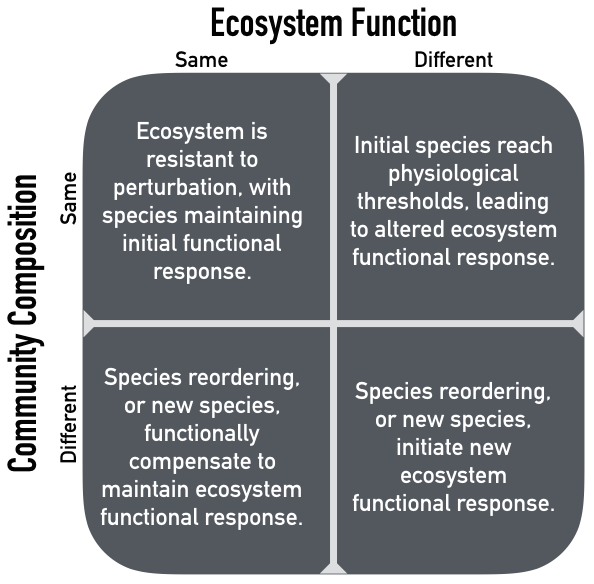
\includegraphics[width=4in]{../figures/hypothesis_figtable.png}
  \caption{Possible outcomes of chronic resource alteration.}
\end{figure}

\newpage{}

\begin{figure}[!ht]
  \centering
      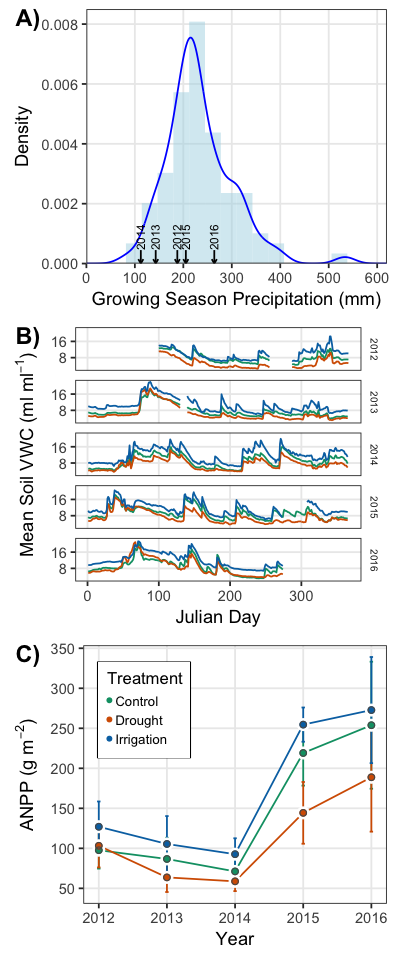
\includegraphics[height=7in]{../figures/data_panels.png}
  \caption{(A) Probability density of historical precipitation from 1926-2016, with the years of the experiment shown with arrows on the \emph{x}-axis. (B) Observed soil volumetric water content (VWC) over the course of the experiment. (C) Mean (points) ANPP and its standard deviation (error bars) for each year of the experiment.}
\end{figure}

\newpage{}

\begin{figure}[!ht]
  \centering
      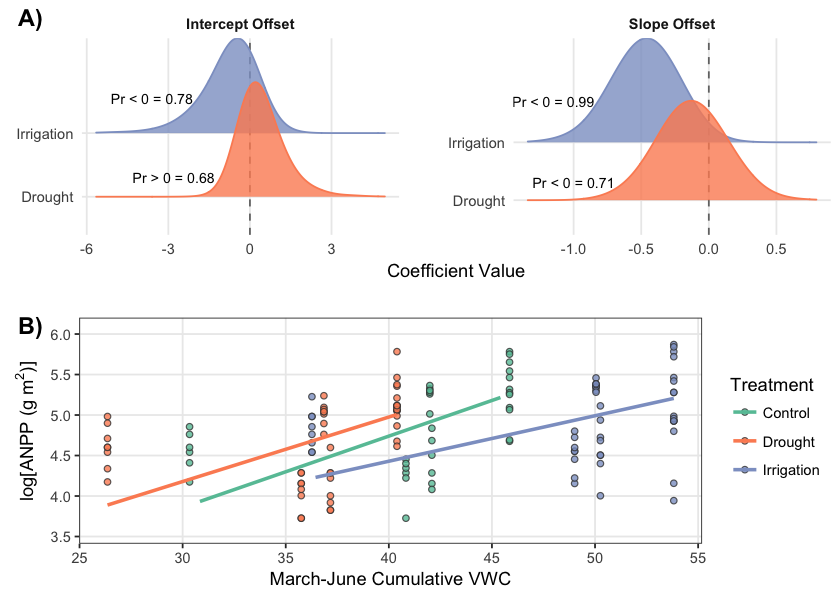
\includegraphics[width=5in]{../figures/glmm_main_results.png}
  \caption{Results from the generalized linear mixed effects model. (A) Posterior distributions of the intercept and slope offsets for the drought and irrigation treatments. Offsets indicate the amount to which the coefficients for drought or irrigation treatments differ from the control treatment estimates. Probabilities (``Pr $<$ 0 ='') for each distribution indicate the probability that coefficient is less than zero. Probabilities greater than 0.95 indicate strong support for the coefficient being less than zero. We only show the one-tailed probability for the value being less than zero because the median of each distribution is less than zero. Kernel bandwidths of posterior densities were adjusted by a factor of 5 for visual clarity. (B) Scatterplot of the data and model estimates shown a solid lines. Model estimates come from treatment level coefficients (colored lines). Note that we show log(ANPP) on the \emph{y}-axis of panel B; this same plot can be seen on the arithmetic scale in supporting material Fig. A2-1.}
\end{figure}

\newpage{}

\begin{figure}[!ht]
  \centering
      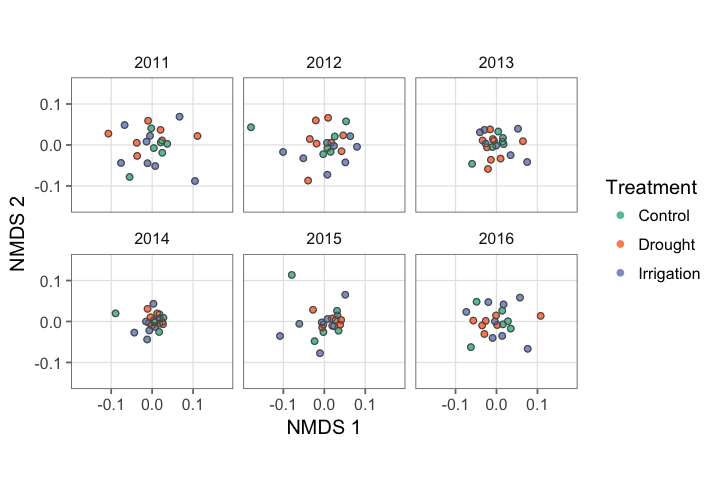
\includegraphics[width=5in]{../figures/sppcomp_bray_all.png}
  \caption{Nonmetric multidimensional scaling scores representing plant communities in each plot, colored by treatment.}
\end{figure}

\newpage{}


\bibliography{/Users/atredenn/Dropbox/Bibliography/usses_water.bib}


\end{document}
